%%\documentclass[a4paper,12pt,oneside]{llncs}
\documentclass[12pt,letterpaper]{article}
\usepackage[right=2cm,left=3cm,top=2cm,bottom=2cm,headsep=0cm]{geometry}

%%%%%%%%%%%%%%%%%%%%%%%%%%%%%%%%%%%%%%%%%%%%%%%%%%%%%%%%%%%
%% Juego de caracteres usado en el archivo fuente: UTF-8
\usepackage{ucs}
\usepackage[utf8x]{inputenc}

%%%%%%%%%%%%%%%%%%%%%%%%%%%%%%%%%%%%%%%%%%%%%%%%%%%%%%%%%%%
%% Juego de caracteres usado en la salida dvi
%% Otra posibilidad: \usepackage{t1enc}
\usepackage[T1]{fontenc}

%%%%%%%%%%%%%%%%%%%%%%%%%%%%%%%%%%%%%%%%%%%%%%%%%%%%%%%%%%%
%% Ajusta maergenes para a4
%\usepackage{a4wide}

%%%%%%%%%%%%%%%%%%%%%%%%%%%%%%%%%%%%%%%%%%%%%%%%%%%%%%%%%%%
%% Uso fuente postscript times, para que los ps y pdf queden y pequeños...
\usepackage{times}

%%%%%%%%%%%%%%%%%%%%%%%%%%%%%%%%%%%%%%%%%%%%%%%%%%%%%%%%%%%
%% Posibilidad de hipertexto (especialmente en pdf)
%\usepackage{hyperref}
\usepackage[bookmarks = true, colorlinks=true, linkcolor = black, citecolor = black, menucolor = black, urlcolor = black]{hyperref}

%%%%%%%%%%%%%%%%%%%%%%%%%%%%%%%%%%%%%%%%%%%%%%%%%%%%%%%%%%%
%% Graficos 
\usepackage{graphics,graphicx}

%%%%%%%%%%%%%%%%%%%%%%%%%%%%%%%%%%%%%%%%%%%%%%%%%%%%%%%%%%%
%% Ciertos caracteres "raros"...
\usepackage{latexsym}

%%%%%%%%%%%%%%%%%%%%%%%%%%%%%%%%%%%%%%%%%%%%%%%%%%%%%%%%%%%
%% Matematicas aun más fuertes (american math dociety)
\usepackage{amsmath}

%%%%%%%%%%%%%%%%%%%%%%%%%%%%%%%%%%%%%%%%%%%%%%%%%%%%%%%%%%%
\usepackage{multirow} % para las tablas
\usepackage[spanish,es-tabla]{babel}

%%%%%%%%%%%%%%%%%%%%%%%%%%%%%%%%%%%%%%%%%%%%%%%%%%%%%%%%%%%
%% Fuentes matematicas lo mas compatibles posibles con postscript (times)
%% (Esto no funciona para todos los simbolos pero reduce mucho el tamaño del
%% pdf si hay muchas matamaticas....
\usepackage{mathptm}

%%% VARIOS:
%\usepackage{slashbox}
\usepackage{verbatim}
\usepackage{array}
\usepackage{listings}
\usepackage{multirow}

%% MARCA DE AGUA
%% Este package de "draft copy" NO funciona con pdflatex
%%\usepackage{draftcopy}
%% Este package de "draft copy" SI funciona con pdflatex
%%%\usepackage{pdfdraftcopy}
%%%%%%%%%%%%%%%%%%%%%%%%%%%%%%%%%%%%%%%%%%%%%%%%%%%%%%%%%%%
%% Indenteacion en español...
\usepackage[spanish]{babel}

\usepackage{listings}
% Para escribir código en C
% \begin{lstlisting}[language=C]
% #include <stdio.h>
% int main(int argc, char* argv[]) {
% puts("Hola mundo!");
% }
% \end{lstlisting}


\title{Análisis3}
\author{Jesús Rodríguez Heras}

\begin{document}
	
	\maketitle
	\begin{abstract} %Poner esto en todas las prácticas de PCTR
		\begin{center}
			Resultado gráfico del SpeedUp del problema 4 de la práctica 6.
		\end{center}
	\end{abstract}
	\thispagestyle{empty}
	\newpage
	
%	\tableofcontents
%	\newpage
	
	%%\listoftables
	%%\newpage
	
	%%\listoffigures
	%%\newpage
	
	%%%% REAL WORK BEGINS HERE:
	
	%%Configuracion del paquete listings
	\lstset{language=bash, numbers=left, numberstyle=\tiny, numbersep=10pt, firstnumber=1, stepnumber=1, basicstyle=\small\ttfamily, tabsize=1, extendedchars=true, inputencoding=latin1}


\begin{center}
	\begin{table}[htbp]
		\begin{center}
			\begin{tabular}{|c|c|c|c|}
				\hline
				\textbf{Elementos} & \textbf{resImagen} & \textbf{resImagenParFin} & \textbf{resImagenParGru}  \\
				\hline 
				$50$ & 0.001 & 0.325 & 0.002 \\ \hline
				$100$ & 0.002 & 2.17 & 0.004 \\ \hline
				$150$ & 0.006 & \texttt{ERROR} & 0.008 \\ \hline
				$200$ & 0.008 & \texttt{ERROR} & 0.007 \\ \hline
				$250$ & 0.014 & \texttt{ERROR} & 0.011 \\ \hline
			\end{tabular}
			\caption{Valores en segundos del tiempo usado por cada algoritmo.}
			\label{tabla:Valores en segundos del tiempo usado por cada algoritmo}
		\end{center}
	\end{table}
\end{center}

\begin{figure}[h]
	\begin{center}
		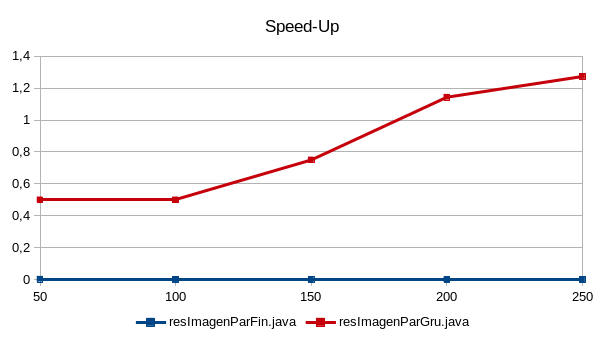
\includegraphics[scale=1]{SpeedUp2.png}
		\caption{Valores del SpeedUp.}
		\label{fig:Valores del SpeedUp}
	\end{center}
\end{figure}
Para la realización de la gráfica, hemos tenido en cuenta dichos datos tomados del tiempo de ejecución de los algoritmos de grano fino (\texttt{resImagenParFin.java}) y de grano grueso (\texttt{resImagenParGru.java}) respecto del algoritmo secuencial (\texttt{resImagen.java}).

Como podemos apreciar en la imagen, el Speed-Up no empieza a ser igual a $1$ hasta un tamaño de matriz de  $200x200$ por parte del algoritmo de grano grueso y, de ahí en adelante, siempre llevará irá a la cabeza, en contraposición al algoritmo de grano fino que irá empeorando su tiempo respecto del secuencial.

Tal como vemos en la gráfica y en la tabla de tiempos, podemos observar como ni siquiera es capaz de ejecutarse para una matriz de tamaño $150x150$ debido a que sobrepasa la memoria del heap de la máquina virtual de java. Ni siquiera cambiando dicha memoria con el flag \texttt{-Xss1024m} hemos podido conseguir que ejecute.

Por lo tanto, podemos deducir que crear muchos hilos no nos asegura en ningún momento una mayor optimización del problema ya que, como se puede ver, la versión secuencial es mejor que la de grano fino.

No ocurre así con la versión de grano grueso en la que se dividen la matriz entre los cores disponibles de la máquina y es en esta versión donde se puede observar una mejoría considerable sobre todo en matrices de mayor tamaño.

Para una matriz de tamaño $10000x10000$ la versión secuencial tarda $0.605$ segundos y la versión de grano grueso tarda $0.192$ segundos, consiguiendo un Speed-Up de $3.151$, muy cerca de los 4 cores que usa la máquina en la que se han probado los programas\footnote{Esta prueba no se ha puesto en la tabla ni en la gráfica para no descuadrar los datos ni dar falsos positivos, por eso se encuentra aparte.}.

\end{document}